\chapter{Introduction}\label{ch:introduction}

\section{Optical Microscopy}

The optical microscope is one of the oldest scientific instruments, and continues to be an essential tool for researchers, clinicians, and engineers across many disciplines. Different from spectacles, which use a single lens to provide magnification for one or both eyes, microscopes are typically defined as having two or more refractive surfaces to provide magnification between the object of interest and the imaging plane, enabling the user to see things much smaller than the normal optical resolution of the human eye. Credit for the inventor of the compound microscope is generally attributed to Hans and Zacharias Jansen of the Netherlands, although the first published work on microscope design wasn't released until 1665 (Hooke and van Leeuwenhoek) \cite{natureMilestones,hookeMicrographica}. In this work, our discussion of microscopes will be limited to optical microscopes - those which are designed for use with light within the optical band of the electro-magnetic spectrum ($390nm \leq \lambda \leq 700nm$), which is approximately the electromagnetic spectrum detectable by the human eye.

\subsection{Imaging and Resolution}
Generally speaking, a single lens may be used to form a magnified image of a sample - this situation is described by the imaging condition,

\begin{equation}
\frac{1}{f} = \frac{1}{s_o} + \frac{1}{s_i}
\end{equation}

Which relates the distance of an optical element to a object under observation $s_o$ to the distance of a conjugate image $s_i$, which may be magnified by a factor $M = \frac{-s_i}{s_o}$ based on the relative distances of each quantity. The variable $f$ corresponds to the focal length of the element, which may also be an effective focal length from the combination of several refractive elements. While this optical system will magnify an object if $M > 1$, it is practically limited to smaller magnifications since there is normally a practical upper limit on $s_o$ (set by working distance) and a lower limit on the distance of the image from the lens $s_i$ (due to eyepiece design).

A compound microscope uses multiple refractive elements to form an image. Typically, the exact number and design of these components is abstracted to the end-user, and can be defined by a relatively low number of descriptive quantities despite the complex internal lens design of a modern microscope objective. Magnification and Numerical Aperture (NA) are the most important of these physical quantities; the magnification of an objective sets the field of view which is relayed by the optic, while the numerical aperture sets a minimum bound on the diffraction-limited resolution. The Numerical Aperture is defined by the formula $NA=n\sin (\theta)$, where $n$ is the refractive index of the medium, and $\theta$ is the maximum half-angle at which light may pass through the objective relative to the radial (optical) axis. The angular dependence of Numerical Aperture is completely described by interference effects which arise from the wave-optics model of light propagation. As multiple off-axis sources of the same wavelength converge to a point, the wavefronts of these sources will cause constructive and destructive interference; The minimum distance between two peaks formed by constructive interference is proportional to both the wavelength of the illumination and the angular separation between the two beams (which is set by the maximum NA of the source). Practically, the size of this spot defines the resolution of the optical system. By the Rayleigh criteria, the resolution of an optical system is defined as:

\begin{equation}\label{eq:intro:rayleigh}
\Delta x_{min}  = \frac{1.22 \lambda}{(NA_{objective} + NA_{illumination})}
\end{equation}

This quantity defines the minimum separation between two points which can be detected by a system with a circular aperture, and is defined by the distance between the center if the point spread function (PSF) and it's first null. Note that Eq.~\ref{eq:intro:rayleigh} is dependent ono both detection side NA ($NA_{objective}$) and illumination side NA ($NA_{illumination}$). The ratio between these NA, typically denoted as $\sigma = NA_{objective}/NA_{Illumination}$, is commonly referred to as the coherence factor. As $\sigma \longrightarrow 0 $, the illumination becomes spatially coherent, meaning the phase of the illumination wavefront at a given point on the sample can be perfectly described by all other points on the sample. This definition assumes that the light source is composed of spatially distributed statistically uncorrelated emitters - contemporary microscope sources such as halogen and tungsten lamps satisfy this criteria while in k{\"o}hler geometry. As sigma increases, the minimum resolvable feature size decreases, leading to images of higher quality, subject to aliasing affects. However, increasing $\sigma$ beyond 1 does not provide further resolution improvement due to the ballistic light (DC term) is not collected by the objective. This is the working principle of dark-field microscopy. Achieving resolution improvements beyond $2\times NA_{objective}$  require computational imaging techniques such as structured illumination \cite{gustafsson2000surpassing}, localization microscopy~\cite{Rust:06, betzig2006imaging}, or computational super-resolution methods such as ptychography\cite{Zheng2013}.

\subsection{Fourier Optics Description}
The sub-field of Fourier optics provides a theoretical bridge between conventional optics and signal processing. In modern microscopes, digital cameras allow the detection of the Intensity of an optical field using a grid of photodetectors, which readily enables the use of digital signal processing techniques on images formed by a microscope. Fourier optics is especially useful for an optical system configured as a 4$f$ system:

\begin{figure}[tbh]
\centering
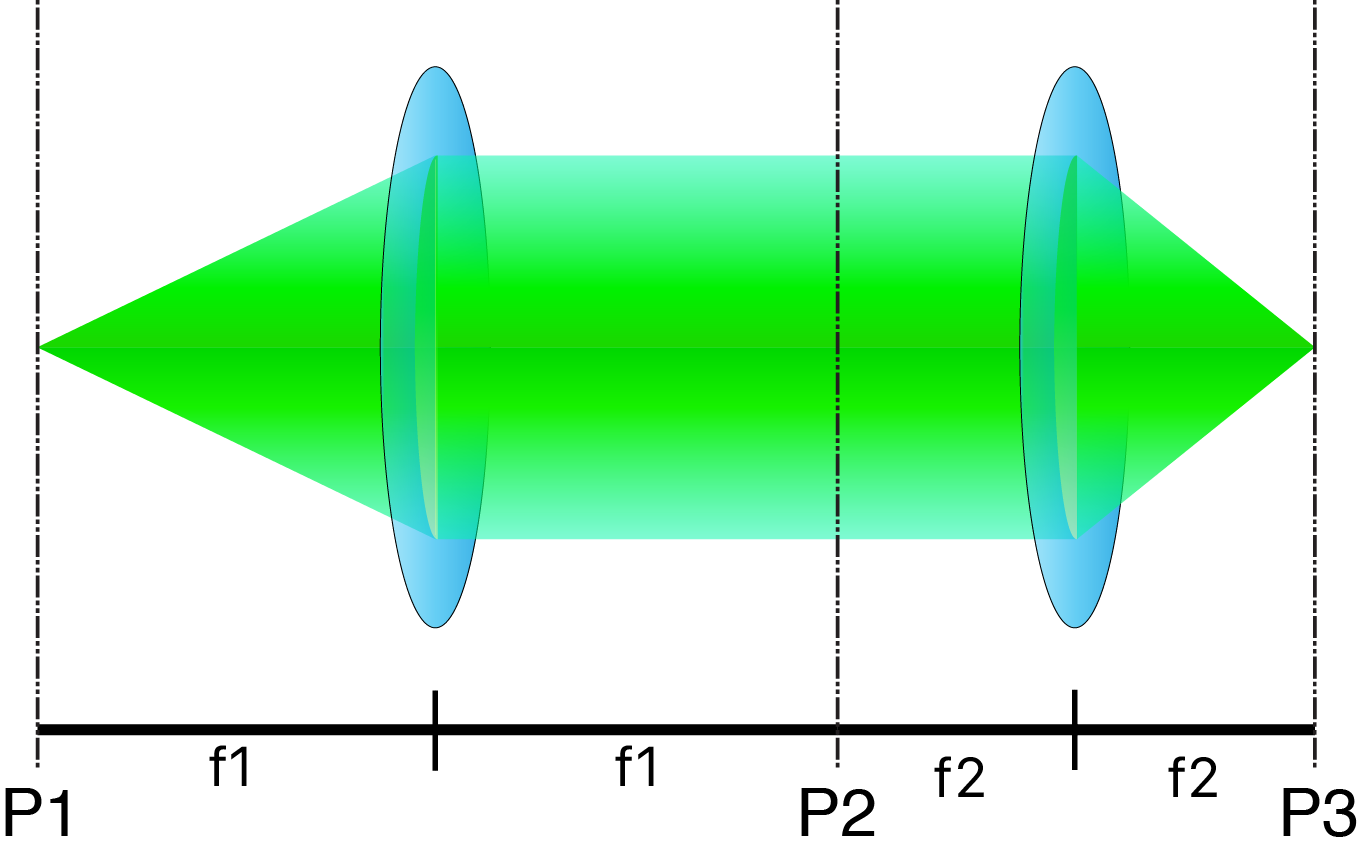
\includegraphics[width=0.4\textwidth]{intro-4f.png}
\caption{\label{fig:4f} Schematic of a 4$f$ optical system}
\end{figure}

In this optical configuration, the lenses in this system operate as forward and inverse Fourier Transform operators on the optical field at P1 up to a given range of support set by the NA of the lens. The Fourier Transform of P1 exists at position P2, which is often occupied by an aperture stop to limit the NA of the objective. This aperture stop prevents stray or highly abberated rays from entering the imaging plane and prevents aliasing, which is a phenomena caused by sampling a signal at a frequency which is below a the Nyquist frequency, defined by the bandwidth of the measurement. In an optical system, this frequency is set by the pixel separation and system magnification relative to the imaging NA of the system.

\section{Computational Microscopy}

\begin{figure}
    \centering
    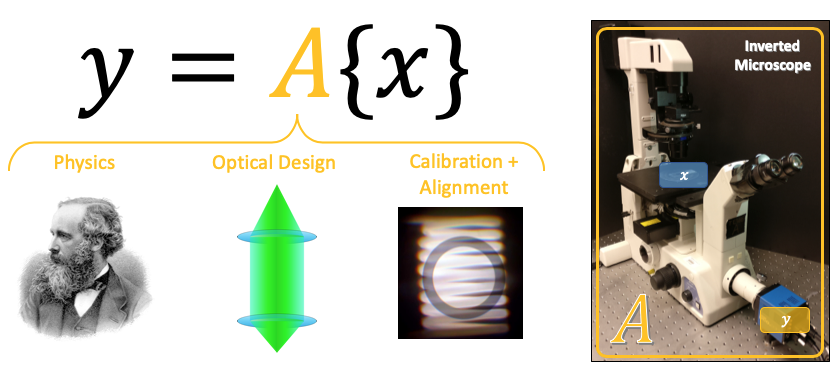
\includegraphics[width=0.95\textwidth]{figures/fig_intro_comp_imaging.png}
    \label{fig:intro_overview}
    \caption{Overview of Computational Imaging. The forward model $\op{A}$ is a function of the physical properties of light, the optical system design, and (mis)calibration of the system. An image of a Nikon TE300 microscope used in this work is provided for context.}
\end{figure}

The concept of using computational tools to simulate and invert optical imaging systems was developed soon after the widespread adoption of computers, and was in some ways a natural extension of the mathematical framework which was developed prior to this time.~\cite{bracewell1986fourier}. The seminal text on imaging using Fourier theory to analyze imaging systems was published in 1968~\cite{goodman:68} which produced the framework which enables many common computational techniques such as deconvolution, which form the backbone of the analysis presented in this work.

Recently, the field of computational imaging has expanded considerably due to increasing availability of computing power and digital sensing hardware. In a Fourier optics model, an optical system can be approximated as a linear system, enabling the application of a large number of algorithms such as least squares, gradient descent, and nonlinear optimization techniques. Computational Imaging takes advantage of this mathematical description to move part of the image formation process from hardware to software. This paradigm enables image formation processes that were previously unfeasible for conventional optical imaging, allowing an optical designer to take advantage of the strengths of both hardware and software during each step of the image formation process. 

An early example of computational imaging was the application of a cubic phase plate at the microscope pupil, which provides drastically increased depth of field but produces a highly distorted image. Since these distortions are known, however, the original image with extended depth of field can be deconvolved using knowledge of the system's point spread function (PSF)\cite{Dowski:95}. Since these early works, computational microscopy has ballooned due to the widespread availability of computing hardware and software tools for simulating optical systems and performing quantitative analysis. Prominent examples include super-resolution methods such as structured illumination~\cite{gustafsson2000surpassing, gustafsson2005nonlinear}, which enhances resolution by projecting a pattern onto the sample, localization microscopy~\cite{betzig2006imaging, Rust:06}, which employs statistical analysis to localize sparse fluorophores using temporal dynamics, and both conventional~\cite{rodenburg2004phase} and Fourier~\cite{Zheng2013} ptychography. Three-dimensional imaging has likewise become a powerful for imaging three dimensional biological quantities, and becomes absolutely necessary for high-$NA$ imaging of thick samples which encounter multiple scattering. Various approaches have been proposed, including deconvolving focal stacks~\cite{agard1984optical}, light-field microscopy~\cite{broxton2013wave, Ng2005}, point-spread function engineering~\cite{pavani2008three}, as well as diffraction tomography~\cite{wolf1969three, kim2014diffraction, maleki1992tomographic}. In addition, computational imaging has been widely used for quantitative phase imaging, using interferometry~\cite{Popescu:06,kim2014diffraction, Bhaduri:12}, Off-axis holography~\cite{Witte:12}, commercial add-ons~\cite{phasics,bon2012method}. Another add-on option uses two cameras to capture defocused images which can then be used to solve the Transport of Intensity Equation (TIE)~\cite{allman2005optical}. Alternatively, if chromatic aberrations are large enough, they can enable single-shot color TIE~\cite{wallerColorTIE} without any hardware changes. 

Many computational imaging problems can be represented as an inverse problem of the form:

\begin{equation}\label{eq:intro_inverse_problem}
\begin{aligned}
& \hat{\vec{x}} = \underset{\vec{\vec{x}}}{\text{argmin}}
& & ||\op{A}\{\vec{x}\} - \vec{y} ||_2^2
\end{aligned}
\end{equation}

Where $\vec{x}$ represents the variable of interest (generally the object), $\op{A}\{\cdot\}$ is the mathematical operation describing the optical system, $\vec{y}$ is the measured intensity, and $\hat{\vec{x}}$ is an estimate of the object $\vec{x}$. The forward operator $\op{A}\{\cdot\}$ is normally formed based on the physics of the optical systems, need not be linear or represented by a matrix.

The goal of a computational imaging system is to invert the forward operator $\op{A}\{\cdot\}$ in a way which minimizes the distance between the object estimate distortions of the forward-inversion process ($||\hat{\vec{x}} - \vec{x}||_2^2$). If $\op{A}\{\cdot\}$ is linear, is can be inverted in a closed-form solution using the Moore-Penrose Pseudo-Inverse~\cite{moore1920reciprocal}, or with an iterative method such as gradient descent. If $\op{A}\{\cdot\}$ is non-linear but smooth, it must be inverted iteratively using analytic expressions for each regularization. If $\op{A}\{\cdot\}$ is non-smooth, it can, in some cases, still be inverted using iterative soft-thresholding method such as FISTA~\cite{beck2009fast}. 

In general, linear problems (characterized by satisfying the relationship $\op{A}\{\vec{a} + \vec{b}\} = \op{A}\{\vec{a}\} + \op{A}\{\vec{b}\} $) are much easier to invert and solve, having lower memory requirements and complexity than other problems as well as a direct inverse. A common subclass of linear forward models are convolutional operators, which apply a blurring function across a measurement. When a convolution is well-posed, it may be efficiently inverted using a FFT-based deconvolution algorithm~\cite{cooley1965algorithm}, which has complexity $N \log(N)$ as opposed to $N^2$ for normal operators.

The performance of inversion processes may be improved by adding regularization term to penalize certain undesirable characteristics of the signal, such as noise. The most commonly used regularization method is Tikhonov (or $\ell_2$) regularization~\cite{tikhonov1943stability}, which enforces a prior on the total energy of a system. Tikhonov regularization is equivalent to adding an additional $\ell_2$ term to Eq.~\ref{eq:intro_inverse_problem}:

\begin{equation}\label{eq:intro_tikhonov}
\begin{aligned}
& \hat{\vec{x}} = \underset{\vec{x}}{\text{argmin}}
& & ||A\{\vec{x}\}-\vec{y} ||_2^2 + \alpha||\vec{x}||_2^2
\end{aligned}
\end{equation}

\noindent where $\alpha$ is a tuning parameter which represents the weight of the Tikhonov prior (normally set to $\frac{1}{SNR}$). If $\op{A}\{\cdot\}$ is linear and can be represented as a matrix, Eq.~\ref{eq:intro_tikhonov} can be directly inverted using a closed-form expression:

\begin{equation}
    \hat{\vec{x}} = ((\mat{A}^H \mat{A})^{-1} + \alpha \mat{I})\mat{A}^H \vec{y}
\end{equation}

\noindent where $\mat{A}$ is the matrix form of $\mat{A}\{\cdot\}$ and $\mat{I}$ is the identity matrix with the same dimensions as $\mat{A}^H \mat{A}$. This closed-form solution makes Tikhonov regularization popular for many inverse problems, although the total energy prior may not be relevant in many cases.

A second commonly used class of priors enforce sparsity of the object in some domain. Mathematically the $\ell_0$ "norm" returns the number of non-zero elements of the input. This norm is non-convex, however, requiring a large combinatorial search which is intractable for most problems~\cite{candes2008enhancing}. As a proxy, the $\ell_1$ norm is conventionally employed as a convex, though non-smooth alternative~\cite{taylor1979deconvolution}. When coupled with a generalized sparsifying operator $\op{W}\{\cdot\}$ and a differential forward model $\op{A}\{\cdot\}$, this problem is convex, and can be written as:

\begin{equation}\label{eq:intro_sparse}
\begin{aligned}
& \hat{\vec{x}} = \underset{\vec{x}}{\text{argmin}}
& & ||\op{A}\{x\}-\vec{y} ||_2^2 + \alpha||\op{W}\{\vec{x}\}||_1
\end{aligned}
\end{equation}

Because the regularization term is non-smooth, iterative solvers must be used to recover the optimal $\hat{\vec{x}}$. When $\op{W}$ is a unitary function $\mat{w}$ (or the identity matrix), a solver implementing proximal gradient descent using soft-thresholding may be used to minimize this objective function, such as FISTA~\cite{beck2009fast}, ADMM~\cite{boyd2011distributed}, or TwIST~\cite{bioucas2007new}. In general, $\mat{W}$ can be any unitary transform, including the Fourier Transform or Wavelet Transform, or a learned unitary operator which is optimized using a machine-learning framework~\cite{ravishankar2013learning}. In all of these cases, the optimal $\hat{\vec{x}}$ may be recovered by performing many iterations of proximal gradient descent:

\begin{equation}
    \vec{x}^{k+1} = \mat{W}^H prox_{\alpha}(\mat{W} (\vec{x}^{k} - \alpha \nabla_{\op{A}\{\vec{x}\}} (\op{A}\{\vec{x}\} - \vec{y})))
\end{equation}

In the case where $\mat{W}$ is not unitary, the above relationship does not hold, and other proximal methods must be used. One prominent example is total-variation regularization (TV), which enforces sparsity of the image gradients~\cite{rudin1992nonlinear}. TV regularization can be implemented using ADMM~\cite{wahlberg2012admm}, FISTA~\cite{beck2009fast}, or using soft-thresholding on wavelet coefficients~\cite{kamilov2012wavelet}, although it is known to create a "cartoon-like" effect for high $\alpha$ values.

\section{Noise in Computational Microscopy Systems}\label{sec:intro_noise}
All measurements contain noise from various sources, including photon quantization, camera electronics. In general, these noise sources can be additive or multiplicative, and may take on a variety of statistical profiles including Gaussian and Poisson distributions. In this work, we generally assume the presence of an additive, Gaussian noise term $\vec{\eta}$ with zero-mean, and variance $\sigma_{\vec{\eta}}$, which is added to each measurement made under a general forward operator $\op{A}\{\cdot\}$:

\begin{equation}\label{eq:intro_forward_model}
    \vec{y} = \op{A}\{\vec{x}\} + \vec{\eta}
\end{equation}

This approximation is generally valid for measurements made with more than 10 photon counts, which includes every case presented in this work (including fluorescence imaging). The effect of this noise on image quality is generally represented as the signal-to-noise ratio (SNR):

\begin{equation}
    \label{eq:intro_snr}
    SNR = \frac{\bar{\vec{y}}}{\sigma_{\vec{\eta}}}
\end{equation}

When inverting the forward operator $\op{A}\{\}$ to recover $\vec{x}$, the presence of $\vec{\eta}$ will lead to error in the measurements. Take, for example, if $\op{A}$ can be represented as a matrix $\mat{A}$, the Moore-Penrose pseudoinverse of the object is given by:

\begin{equation}\label{eq:intro_noise_inverse}
        \hat{\vec{\vec{x}}} = (\mat{A}^H \mat{A})^{-1} \mat{A}^H y = (\mat{A}^H \mat{A})^{-1} \mat{A}^H \mat{A} \vec{x} + (\mat{A}^H \mat{A})^{-1} \mat{A}^H \vec{\eta} = \vec{x} + (\mat{A}^H \mat{A})^{-1} \mat{A}^H \vec{\eta}
\end{equation}

Based on Eq.~\ref{eq:intro_noise_inverse}, the error between $\hat{\vec{x}}$ and the true $\vec{x}$ is $(\mat{A}^H \mat{A})^{-1} \mat{A}^H \vec{\eta}$. Taking the covariance of this term, we can find an expression for the covariance of the error term in the reconstruction:

\begin{equation}\label{eq:intro_noise_covariance}
    \mat{\Sigma}_{\mat{A}^{\dagger}\vec{\eta}} = (\mat{A}^H \mat{A})^{-1} \mat{A}^H \sigma_{\vec{\eta}}^2 \mat{A} (\mat{A}^H \mat{A}) ^{-H} = \sigma_{\vec{\eta}}^2 (\mat{A}^H \mat{A})^{−1} \mat{A}^H  \mat{A} (\mat{A}^H \mat{A}) ^{-H} = \sigma_{\vec{\eta}}^2 (\mat{A}^H \mat{A}) ^{-H} 
\end{equation}

The main result of Eq.~\ref{eq:intro_noise_covariance} is that the inversion process re-weighs, or "colors" the original Gaussian white noise $\vec{\eta}$. When $\mat{A}$ has an $\ell_2$ operator norm of 1, the minimum singular value of $\mat{A}$ defines the maximum noise amplification, while the sum of the inverse singular values defines the total RMSE:

\begin{equation}\label{eq:intro_noise_amplification}
    \sigma_{\mat{A}^{\dagger}\vec{\eta}} = \sigma_{\vec{\eta}} \sqrt{\mat{\Sigma}_{i=0}^N{\frac{1}{\sigma_i^2\{\mat{A}\}}}} = \sigma_{\vec{\eta}} \sqrt{Tr\{(\mat{A}^H \mat{A})^{-1}\} / N}
\end{equation}

\noindent where $N$ is the length of $\vec{x}$ and $\sigma_i^2 \{\mat{A}\}$ represents the $i^{th}$ singular value of $\mat{A}$. This definition is consistent with~\cite{agrawal2009optimal}.

\section{Coded Illumination for Optical Microscopy}
Since the 16$^{th}$ century microscopes have employed some sort of light source to illuminate a specimen, from candles to semiconductor light sources. In this work, we explore, through both theory and demonstration, the use of programmable LED sources for microscopy, replacing conventional sources such as halogen lamps. These sources enable both fast switching of qualitative contrast methods~\cite{Zheng2011, albeanu2008led} as well as the capability to perform quantitative reconstructions of the complete complex field of the sample~\cite{Tian3dDpc, Zheng2013, tian2015quantitative}.

Contrast in optical microscopy is conventionally obtained in a variety of ways – for purely absorptive samples, bright field microscopy images the light that is attenuated by the sample by illuminating within the range of angles defined by the numerical aperture ($NA$) of the objective. Conversely, dark field microscopy uses illumination from angles outside of the illumination $NA$, imaging only light that is scattered or “bent” by a refractive medium such as water. Rather than relying on expensive illumination hardware to block transmitted light at the pupil plane, the simple addition of an LED array enables both of these modalities by dynamically changing the pattern via software~\cite{Zheng2011, zijiMulti}.

% TODO: figure for this

In addition to qualitative phase contrast, computational illumination using a LED array enables quantitative phase recovery through with an LED array microscopy involves methods such as Fourier ptychography Ptychography~\cite{Zheng2013, Tian14} and differential phase contrast~\cite{mehta2009quantitative,
tian2015quantitative}, enabling the measurement of the dry mass of many aqueous biological samples~\cite{popescu2008imaging, popescu2008optical}. 

In the following chapters, I will describe several novel applications and of coded imaging in optical microscopy, as well as fabrication methods for coded illumination devices and self-calibration techniques for the aforementioned methods. Chapter 2 describes methods for qualitative and quantitative phase recovery, including single-shot quantitative phase imaging method which uses partially coherent color illumination to recover the complete optical field of an object from a single measurement. In addition, we perform a SNR-based optimization of LED patterns for linearized phase retrieval using a partially coherent source. Chapter 3 describes a novel method for recovering a large field-of view with SNR. Here, we introduce motion deblur into each measurement, and use a motion deblurring algorithm to recover an object's complete optical field as it moves across the field of view. We demonstrate the use of this technique for brightfield imaging, fluorescence imaging, and quantitative phase imaging, including an analysis of optimal acquisition strategy in terms of SNR. In Chapter 4, we describe the fabrication of several prototypes used for coded illumination, including a programmable domed LED array, LED sources for high-throughput imaging, as well as Computational CellScope, a prototype device which uses a programmable domed LED illumination to perform quantitative phase imaging, digital refocusing, and multi-contrast imaging in a portable package, where all acquisition and post-processing is performed on a smartphone. Chapter 6 describes self-calibration techniques for quantitative phase imaging, including LED position recovery for LED domes, and aberration recovery using a linearized model. These methods are essential for practical implementation of many quantitative phase imaging techniques. Chapter 5 concludes this dissertation on quantitative microscopy using coded illumination, and provides future extensions of the work presented in the previous chapters. Fig.~\ref{fig:intro_system_dome} shows the system which was used in most experiments presented in this work.

\begin{figure}
    \centering
    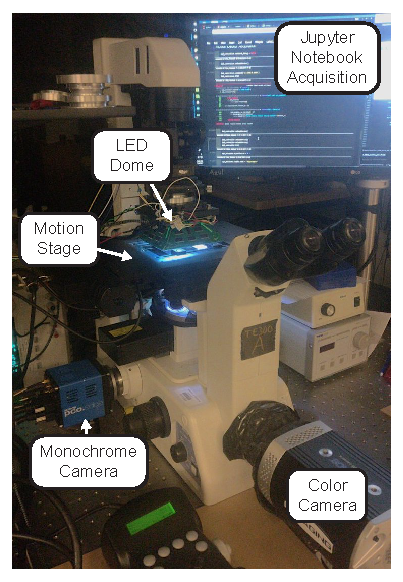
\includegraphics[width=0.6\textwidth]{figures/fig_intro_dome_system.pdf}
    \label{fig:intro_system_dome}
    \caption{Nikon TE300-based system used for most experiments presented in this work. This configurations is configured both color and monochrome cameras, although in practice either may be used. A quasi-domed illuminator is mounted in place of the conventional optical condenser, although this may be replaced with a single LED high-throughput imaging.}
\end{figure}